\documentclass[11pt,openright,a4paper]{report}
%%
%% This document template assumes you will use pdflatex.  If you are using
%% latex and dvipdfm to translate to pdf, insert dvipdfm into the options.
%%


%%
%% Package includes to provide the basic style
%%
\usepackage{graphicx}   % Permits import of various graphics formats
\graphicspath{{../img/}}
\usepackage{hyperref}   % Provides hyperlinks to sections automatically
\usepackage{pdflscape}  % Provides landscape mode for end code listings
\usepackage{multicol}   % Provides ability to split output into columns
\usepackage{listings}   % Provides styled code listings
\usepackage[left=3.5cm, right=2.5cm, top=3.5cm, bottom=3cm]{geometry} % Margins
\usepackage{titlesec}
\usepackage{lipsum}
\usepackage[numbers]{natbib}
\usepackage{enumerate}
\usepackage{tabularx}
\usepackage{longtable}
\usepackage{pgfgantt}
\usepackage{wrapfig}
\usepackage{amsmath, amsthm, amsfonts}
\newtheorem{definition}{Definition}
\usepackage{bbm}
\usepackage[shortlabels]{enumitem}
\usepackage{appendix}
\usepackage{todonotes}

\newcommand\requirement[2]{
  {#1} %\textbf{Priority: {#2}.}
}

\newcommand\invisiblesubsection[1]{
  \refstepcounter{subsection}
  \addcontentsline{toc}{subsection}{\protect\numberline{\thesubsection}#1}
  \subsectionmark{#1}}
\makeatother

\newcommand{\possessivecite}[1]{\citeauthor{#1}'s \citeyear{#1}}

  
%%
%% Set some page size changes from the standard article class
%%
\usepackage{calc}
\setlength{\parskip}{6pt}
\setlength{\parindent}{0pt}
\addtolength{\hoffset}{-0.5cm}
%\addtolength{\textwidth}{2.5cm}
\titleformat{\chapter}[display]{\vspace{-2cm}\normalfont\bfseries}{}{0pt}{\huge}

%%
%% Format definitions for the style
%%
%\usepackage{harvard}    % Uses harvard style referencing
\bibliographystyle{agsm}%{alpha}
\setcitestyle{authoryear}
%\citationstyle{dcu}
\pagestyle{headings}
\fussy



%%
%% Helpers
%% 
\usepackage[final]{pdfpages}
%\setcounter{secnumdepth}{4}


%%
%% Definitions to provide layout in the dissertation title pages
%%
\newenvironment{spaced}[1]
  {\begin{minipage}[c]{\textwidth}\vspace{#1}}
  {\end{minipage}}


\newenvironment{centrespaced}[2]
  {\begin{center}\begin{minipage}[c]{#1}\vspace{#2}}
  {\end{minipage}\end{center}}


\newcommand{\declaration}[2]{
  \thispagestyle{empty}
  \begin{spaced}{4em}
    \begin{center}
      \LARGE\textbf{#1}
    \end{center}
  \end{spaced}
  \begin{spaced}{3em}
    \begin{center}
      Submitted by: #2
    \end{center}
  \end{spaced}
  \begin{spaced}{5em}
    \section*{COPYRIGHT}

    Attention is drawn to the fact that copyright of this dissertation rests
    with its author. The Intellectual Property Rights of the products
    produced as part of the project belong to the author unless otherwise specified
    below, in accordance with the University of Bath's policy on intellectual property 
   (see http://www.bath.ac.uk/ordinances/22.pdf).

    This copy of the dissertation has been supplied on condition that anyone
    who consults it is understood to recognise that its copyright rests with its
    author and that no quotation from the dissertation and no information
    derived from it may be published without the prior written consent of
    the author.

    \section*{Declaration}
    This dissertation is submitted to the University of Bath in accordance
    with the requirements of the degree of Bachelor of Science in the
    Department of Computer Science. No portion of the work in this dissertation
    has been submitted in support of an application for any other degree
    or qualification of this or any other university or institution of learning.
    Except where specifically acknowledged, it is the work of the author.
  \end{spaced}

  \begin{spaced}{5em}
    Signed: \vspace{1cm}
\includegraphics[width=3cm]{img/signature.png}
  \end{spaced}}
  



\newcommand{\consultation}[1]{%
\thispagestyle{empty}
\begin{centrespaced}{0.8\textwidth}{0.4\textheight}
\ifnum #1 = 0
This dissertation may be made available for consultation within the
University Library and may be photocopied or lent to other libraries
for the purposes of consultation.
\else
This dissertation may not be consulted, photocopied or lent to other
libraries without the permission of the author for #1 
\ifnum #1 = 1
year
\else
years
\fi
from the date of submission of the dissertation.
\fi
\vspace{4em}

Signed: 
\includegraphics[width=3cm]{img/signature.png}
\end{centrespaced}
}


\usepackage{epigraph}
%\epigraphsize{\small}
\setlength\epigraphwidth{13cm}
\setlength\epigraphrule{0pt}

\usepackage{etoolbox}

\makeatletter
\patchcmd{\epigraph}{\@epitext{#1}}{\itshape\@epitext{#1}}{}{}
\makeatother


%%
%% END OF DEFINITIONS
%%

    %% These are the includes required for the doc 


\title{Automatic Summarisation in Support of Document Triage}
\author{Damask Talary-Brown}
\date{Bachelor of Science in Computer Science with Honours
	\\ The University of Bath
	\\ September 2016 %TODO automate
}

\begin{document}


% Set this to the language you want to use in your code listings (if any)
\lstset{language=Java,breaklines,breakatwhitespace,basicstyle=\small}


\setcounter{page}{0}
\pagenumbering{roman}


\maketitle
\newpage


% Set this to the number of years consultation prohibition, or 0 if no limit
\consultation{0}
\newpage


\declaration{Dissertation title}{Your name}
\newpage


\abstract
Your abstract should appear here.  An abstract is a short
paragraph describing the aims of the project, what was
achieved and what contributions it has made.
\newpage


\tableofcontents
\newpage
\listoffigures
\newpage
\listoftables
\newpage


\chapter*{Acknowledgements}
Add any acknowledgements here.
\newpage


\setcounter{page}{1}
\pagenumbering{arabic}



\chapter{Introduction}
%% Uncomment this to include a separate tex file wih the introduction contents
%\vspace{-0.5cm}
\epigraph{``The Press, Watson, is a most valuable institution, if you only know how to use it."}{--- \textup{Sherlock Holmes}, The Adventure of the Six Napoleons\\[0.2cm] \textup{Sir Arthur Conan Doyle}}

\section*{Why don't we Understand the News?}

The day the result of the 2016 United Kingdom EU Membership Referendum was announced, the \citeauthor{googletrends} reported a 250\% increase in searches for ``What happens if we leave the EU?'' Much like the case of David Leonhardt's 2008 article in the New York Times which began, ``Raise your hand if you don't quite understand this whole financial crisis,'' national news commentary had focused on little else in the preceding months.

Some months after Leonhardt's article was published, Journalism Professor Jay Rosen voiced his agreement with its premise in a blog post on the failure of journalism during the financial crisis; ``there are certain very important stories -- and the mortgage crisis is a good example -- where until I grasp the whole I am unable to make sense of any part.''\citep{NationalExplainer}

Studies have found that the general public use news media to make important life decisions, for entertainment and discussion, as a requirement of their jobs, and out of perceived civic obligation \citep{InformationCartography,UnderstandingTheParticipatoryNewsConsumer}. As a result of the ongoing shift towards online multimedia journalism, there has been an explosion of globally accessible knowledge which is expanding at an unprecedented rate as the internet grows. 

Although ubiquitous news media has resulted in more immediate and diverse coverage of current events, the volume of content available online has made the process of understanding it both daunting and off-putting to young adults \citep{anewmodelfornews}. Additionally, while news aggregators and RSS readers make it faster for users to access the news they care about, they do not aid comprehension. In spite of these facts, little attention has been given to addressing the problem that understanding news articles individually is inherently reliant on understanding news articles as a collection. 

Existing information infrastructure has been criticised both for not supporting the cross-correlation between collections of related news articles \citep{GalaxyOfNews}, and for attempting fit complex narratives into reductive and misleading visualisations \citep{InformationCartography}. Research into how humans' spatio-cognitive abilities can be applied to more abstract visual metaphors \citep{FromMetaphorToMethod} suggests the strength of visual metaphors lies in their familiarity. We therefore build on the work of \cite{GeneratingInformationMaps} to integrate the Metro Map metaphor into the news aggregation process.

\section*{Key Aims and Contributions}
The primary aim of this project is the development of a tool which generates interactive metro maps of news from RSS feeds, with individual articles transformed into stations and common themes transformed into \textit{metro lines}. Our goal is to reduce the information overload experienced by news consumers by providing contextual links between articles and topics.

The resultant system is a news feed aggregator with graphically structured output, and to the best of our knowledge is first of its kind. Contributions of this dissertation include:\vspace{-0.3cm}
\begin{itemize}[itemsep=0.1em]
	\item Implementation of efficient keyword extraction using tf-idf \citep{tfidf} on a reduced keyword space of named entities (Section \ref{sec:keys}).
	\item A novel and lightweight method for performing entity disambiguation within current events articles using Google's Knowledge Graph API (Section \ref{sec:gkg}).
	\item Formalisation of the metrics \textit{Line Coverage} and \textit{Affinity} as criteria for evaluating and ranking candidate metro lines (Sections \ref{sec:linecoverage} and \ref{sec:affinity}).
	\item Recommendations for how D3.js parameters can be manually tuned to generate initial force-directed station positions for planar embeddings of metro maps (Section \ref{sec:fdp}).
	\item The first application of \citeauthor{AutomaticMetroMapLayoutThesis}'s [\citeyear{AutomaticMetroMapLayoutThesis, AutomaticMetroMapLayout}] aesthetic criteria for metro maps to maps drawn from news corpora (Section \ref{sec:stottapplication}).
	\item An empirical evaluation which provides statistical evidence to support the hypothesis that users recall more topics after using our metro maps than after reading news structured as a chronological list (Chapter \ref{c:conclusions}). 
\end{itemize}
 

\section*{Outline}
The structure of this dissertation is as follows: \vspace{-0.1cm}
\begin{description}[leftmargin=5.58em,style=nextline]
	\item [Chapter \ref{c:litreview}] provides an overview of the background literature upon which this project relies, including an introduction to information overload and sensemaking, and a justification of appropriate visualisations for news corpora.
	\item [Chapter \ref{c:reqs}] describes the scoping of the system, the informal requirements gathering process undertaken, and the rationale behind the significant design decisions made.
	\item [Chapter \ref{c:implementation}] discusses the algorithms and techniques chosen to transform the data from feed to visualisation, describes how they were implemented in the system and explains the trade-offs which were encountered.
	\item [Chapter \ref{c:results}] provides a set of example results generated by the system from different RSS feeds and analyses them from the perspectives of content, layout, and context.
	\item [Chapter \ref{c:evaluation}] describes the process by which we evaluated the system in a two-part user study and discusses the results and implications of our experiments.
	\item [Chapter \ref{c:conclusions}] summarises both the contributions and limitations of this work, and provides a discussion on future research directions.
\end{description}



This is the introductory chapter.

\section{Example Section}
Like all chapters, it will have a number of sections

\subsection{Example Subsection}
\ldots and sub-sections

\subsubsection{Example sub-subsection}
\ldots and sub-subsections.

\begin{table}[htb]
\begin{center}
\caption{An example table}
\label{Example-Table}
\begin{tabular}{|l|l|}
\hline
Items & Values \\
\hline
\hline
Item 1 & Value 1 \\
Item 2 & Value 2 \\
\hline
\end{tabular}
\end{center}
\end{table}

\section[short section title]{Another section}
Another section, just for good measure.
You can referene a table, figure or equation using \verb|\ref|, just
like this reference to table \ref{Example-Table}.

\section{Example lists}

\subsection{Enumerated}

\begin{enumerate}
\item Example enumerated list
  \begin{itemize}
  \item a nested enumerated list item
  \end{itemize}
\item Second item in the list
\end{enumerate}

\subsection{Itemized}

\begin{itemize}
\item Example itemized list
  \begin{itemize}
  \item a nested itemized list item
  \end{itemize}
\item Second item in the list
\end{itemize}

\subsection{Description}

\begin{description}
\item[Item 1] Example description list
\item[Item 2] Second item in the list
\end{description}


\chapter{Literature Survey}
%% Uncomment this to include a separate tex file wih the introduction contents
%\section{Why don't we Understand the News?}

The day the result of the 2016 United Kingdom EU Membership Referendum was announced, the \citeauthor{googletrends} reported a 250\% increase in searches for ``What happens if we leave the EU?'' Much like the case of David Leonhardt's 2008 article in the New York Times in which began, ``Raise your hand if you don't quite understand this whole financial crisis,'' national news commentary had focused on little else in the preceding months.

Some months after Leonhardt's article was published, Journalism Professor Jay Rosen voiced his agreement with its premise in a blog post on the failure of journalism during the financial crisis; ``there are certain very important stories -- and the mortgage crisis is a good example -- where until I grasp the whole I am unable to make sense of any part.''\citep{NationalExplainer} 

It has become apparent that prolific coverage alone is not enough to engage and support the public in understanding the complexities of current events. Historically, news media has been limited in the volume of content it can produce by physical constraints such as printing costs, but the rise of the internet as a platform to deliver it has lead to an explosion of content, both through existing media channels and through competing social media websites and blogs. 

The term \textit{ambient news} was coined by \citet{newnewsoldnews} to describe the ubiquity of news in the current information landscape. Others have commented in a more critical light; describing the proliferation of competing news media as ``as pervasive--and in some ways as invasive--as advertising.'' \citep[p.2]{overloadjournalismsbattle}


In \citeyear{anewmodelfornews}, The Associated Press conducted an extensive field study  into the news consumption habits of young adults. Among their key findings were three points which acutely summarise the news overload problem;
\begin{itemize}
	\item \textbf{``Consumers are experiencing news fatigue.''} \par
	The study found participants were debilitated and overwhelmed, and that their levels of dissatisfaction lead to a decrease in the effort they put into news acquisition. This is consistent with multiple other studies \citep{newsandtheoverloadedcustomer, UnderstandingTheParticipatoryNewsConsumer, InformationAccessinComplexPoorlyStructuredInformationSpaces} which found participants across every demographic were overwhelmed by the amount of news content available to them and agreed that it prevented them exploring news on less familiar topics.\\ 
	
	\item \textbf{``Story resolution is key.''} \par
	Participants' consistent enjoyment of sports and entertainment news was due in part to the formulaic storytelling which characterises these types of journalism, with clear chronology to provide contextual back story. The feeling of enjoyment gained from reading procedural stories directly contrasts with what the same participants experienced reading World news, where they struggled to find resolution to stories which were unfolding at the time.
	
	\item \textbf{``Consumers want depth but aren't getting it''} \par
	It was observed that participants, in their efforts to discover \textit{below-the-fold} content (defined in the context of the AP's model, \citeyear[p.37]{anewmodelfornews}) from particular headlines, often found themselves reading the same summary-level content from different news sources. It was recommended that news providers support this by ``designing innovative formats and creating easier pathways to deep content.'' \citep[p.49]{anewmodelfornews}
\end{itemize}

Initially, the third point seems to be a direct contradiction to the first; we are overwhelmed by the volume of news we are exposed to, but we also crave more detail from the news we do consume. However, it brings to light the issue of information \textit{quality} as a requirement of news consumers.

 Journalism, and therefore its quality, can be viewed along a spectrum between two models; a model for the communication of facts, and a model for entertainment and storytelling. From the three points above, it is apparent that quality at both ends of the spectrum is being sought, since the desire for quality below-the-fold content is covered by the first model, and the desire for quality story resolution by the second.

\subsection{Information Overload \label{sec:information-overload}}

News fatigue is a domain-specific type of information overload, a phenomenon formally defined as ``when the information processing demands on time to perform interactions and internal calculations exceed the supply or capacity of time available for such processing'' \citep[p.206]{InformationOverloadATemporalApproach}. Information overload is a multifaceted problem which can be modelled as a combination of three contributing factors (Figure \ref{fig:dimensions}).

\begin{figure}[htbp!]
	\centering
	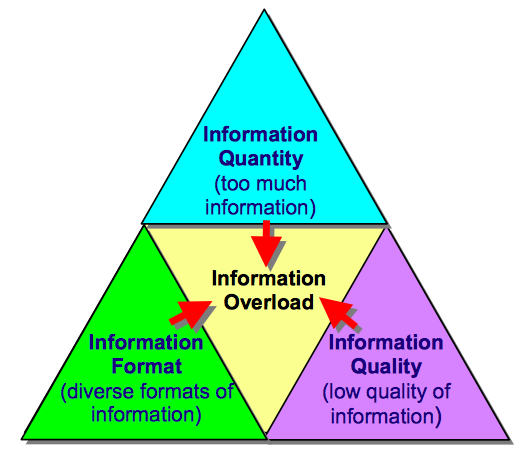
\includegraphics[width=.5\textwidth]{img/lit-survey/overload-model.png}
	\caption{Dimensions of information overload, as defined by \citet{TowardsAnOptimalResolutionToInformationOverload}.}
	\label{fig:dimensions}
\end{figure}

These factors correspond directly to the three points previously identified from the \citeauthor{anewmodelfornews} study. High information quantity leads to news fatigue, information format determines the level of possible story resolution, and information quality determines how much depth a reader can gain from the news they consume. The authors did not find a single solution which could address all three factors, but they did identify information quantity as the most significant contributor to overload.

\citet{GuestEditorsIntroductionInformationOverload} further decompose information quantity into spatial and temporal dimensions in the specific context of news articles. Spatial quantity refers to articles which are near-identical in terms of facts presented being published by different media outlets, and temporal quantity refers to articles on a single topic being published in quick succession over a short period of time. 

Intuitively, the terms spatial and temporal quality seem illogically named, as a set of articles with high spatial quantity would cover a smaller area of information space and vice versa. High spatial quantity will therefore be referred to as \textit{redundancy}, and high temporal quantity as \textit{fragmentation}, since a sudden burst of articles published on the same topic suggests a currently unfolding story being told in parts.

To adequately determine the contributory factors relating to news fatigue, all four dimensions of information overload should be considered, and will therefore be explored in more detail in the following sections.

\subsubsection{Information Quality}
In the context of factual data rather than news specifically, \citet{DataQualityInContext} defined information quality in terms of four components; intrinsic quality, accessibility quality, contextual quality and representational quality. If news can be rationalised to its core function as an interpretation of facts and other raw data such as images, then this same framework can be experimentally applied to news journalism in order to determine which factors could influence its quality.

Intrinsic quality is a measure of the accuracy, objectivity, believability and reputation of data. In the context of news, the first three factors would typically be true for all major news sources, and the reputation would be dependent on whether the article originated from a trusted source or not. Accessibility quality is less relevant to online news media, as it is concerned with data access and security. Contextual quality is the most relevant category in respect to news, concerning timeliness, amount of data, and value-added. In the news domain, this would mean an article's quality is dependent on its performance against a background of other articles; whether or not it contributes anything recent or previously unknown. Finally, representational quality is concerned with ease of understanding and interpretability, which are easily translatable concepts.

The implications of applying the Information Quality Framework \citep{DataQualityInContext} to news articles are that quality may be influenced by the reputation of the source, the timeliness of publication, value-added by the article (i.e. content which couldn't be derived from other sources) and the ease of understanding of the content.

\subsubsection{Information Format}
The domain of news articles is a more specific information space than that of documents in general, and by nature most news articles share some common formatting and structural elements such as headlines, timestamps, and relevant images. As a result of this, it is unlikely that any two articles from popular news providers would be diverse enough in content format to overshadow the information quantity problem.

\subsubsection{Fragmentation (Temporal Quantity)}

The rise of social media sites such as Twitter delivering news to consumers has lead to a high degree of news fragmentation, due to the constraints of the microblogging service's 140-character limit. 24-hour television news paved the way for new formats of real-time content delivery, and the ever-expanding network of online social media channels stepped up to deliver. 

It logically follows from the fragmented nature of real-time news journalism that temporal quality suffers; stories are published and updated intermittently over short periods of time, meaning there is more content for the consumer to piece together in order to understand a story. The fragmentation is somewhat mitigated by Twitter's use of hashtags to denote a Tweet's topics. Hashtags help readers form a coherent and picture of unfolding events from the incremental contributions of thousands of participating users \citep{BlogsTwitterAndBreakingNews}.

\citet{BreakingNewsDetectionAndTrackingInTwitter} developed a methodology to collect and group Tweets on breaking news topics, using hashtags for topic identification or \textit{story-finding}, and grouping similar messages together to form a single news story. Their algorithm for similarity is a function of the tf-idf \citep{TermWeightingApproachesInAutomaticTextRetrieval} of the two messages and the number of named entities they have in common.

\subsubsection{Redundancy (Spatial Quantity)}
It is in the nature of news that newsworthy stories get repeated across multiple sources. When consumers read news on a particular from more than once source, it is likely that they will read variations on the same facts in multiple articles.

Attempts such as \citep{InformationFusionInTheContextOfMultiDocumentSummarization} have been made to synthesise summaries of collections of similar online documents, a practice here termed \textit{information fusion}, with news articles from different sources being given as a specific use-case. However, the process of extracting common sentences between documents was in order to reformulate them into a single summary, rather than to determine the level of similarity between the documents.

A more relevant approach was presented by \cite{UtilizingPhraseSimilarityMeasures}, who used the \textit{title} and \textit{description} attributes of elements in RSS feeds as content descriptors to mitigate the overhead of processing entire documents for phrases. The content descriptors are then used to compute phrase \textit{n}-grams as a measure of similarity between any two documents. The similarities in this case were used to remove subsumed articles and cluster non-redundant similar ones, in order to streamline feed content for readers.

It should be noted that there is an overlap between the notion of spatial quantity and one of the four influencing factors in information quality; contextual quality. If a feed contains two articles which state the same number of identical facts, they therefore contribute to information overload on both the qualitative and quantitative fronts.

Viewing the dimensions of overload from a news domain perspective, it is clear that (consistent with the findings of \citet{TowardsAnOptimalResolutionToInformationOverload}) information quantity is the most relevant contributing factor in respect to fatigue, along factors influencing contextual quality such as value-added and timeliness. Any proposed solutions to the news overload problem should therefore address these factors first.

\subsection{Supporting Sensemaking}

Sensemaking is the basis for forming contextual knowledge; the process by which we incorporate new information into our existing cognitive frameworks, and how we go from reading something to understanding it \citep{FromInformationToKnowing}. In broader terms, \citeauthor{OrganizingAndTheProcessOfSensemaking} describe sensemaking as ``[being] about the question: What does an event mean? In the context of everyday life, when people confront something unintelligible and ask, `What's the story here?'{}'' \citep[p.85]{OrganizingAndTheProcessOfSensemaking} 

This definition relates directly to the news overload problem because one component of sensemaking is the contextual story resolution The \citet{anewmodelfornews} study identified news consumers are craving. It has also been observed that often readers are not interested in specific articles on a subject, and only the thematic content of the topic they belong to \citep{AnalysingUserAccessToAnOnlineNewspaper}. How then, do readers make sense of a collection of articles surrounding a particular topic?

When presented with a large document collection, \citet{BeingLiteratreWithLargeDocumentCollections} found all of their subjects began by clustering the contents into groups which formed a heuristic representation or mental model, used to provide an overview. However, current information infrastructure has been criticised for not supporting the cross-correlation between connected news articles \citep{GalaxyOfNews}.

Writing for the Columbia Journalism review in 2008, \citeauthor{overloadjournalismsbattle} outlined a suggestion for the new roles of journalism in the information era; ``By linking stories to one another and to background information and analysis, news organizations help news consumers find their way through a flood of information that without such mediation could be overwhelming and nearly meaningless''\citep[p.10]{overloadjournalismsbattle}. 

Similarly, \citet{FromInformationToKnowing} make the recommendation in the context of contemporary media consumption that news providers should adapt to an environment of news overload by adding facilities enabling readers to categorise, sort and search news collections. Additional findings of this study suggested that the contextual background provided by having more detailed coverage aids the sensemaking process, as it helps users form links between new information and their existing frameworks, but this presents an interesting conflict with the goal of reducing information overload when considering large collections of documents.

It is apparent that many recommendations have been made from within the field of journalism that at the point of delivery, news content should incorporate contextual links between related articles. This is important both from a sensemaking perspective to emphasise connections, and from an information overload perspective to help users find meaning in an inundated news landscape.

The news overload problem can now be reformulated with scope and detail: How can we display a collection of related news articles in such a way that users are not overwhelmed by unstructured content and are free to explore the underlying contextual pathways?

A simple starting point comes from a familiar idiom; a picture is worth a thousand words.

\section{An Overview of Information Visualisation}

Of course, a picture is not always worth a thousand words, particularly when the picture is unstructured and complex in its own right. However, a recognised and effective technique for bridging the gap between a set of data and a user's mental model and subsequent comprension of the data is information visualisation, or InfoVis. \citep{UnderstandingAndCharacterizingInsights, ThemeRiver}. This section provides a brief overview of a formative InfoVis taxonomy and uses the taxonomy to categorise appropriate visual models for newsfeed visualisation.

In his seminal paper on information visualisation, \citeauthor{TheEyesHaveIt} proposed a taxonomy for visualisations comprising seven data type abstractions, and seven tasks which are components of the visual information seeking mantra; ``Overview first, zoom and filter, then details-on-demand.'' \citep[p.1]{TheEyesHaveIt}

\citeauthor{TheEyesHaveIt}'s type abstractions are as follows:
\begin{description}[leftmargin=11em,style=nextline]
	\item [1-dimensional] Linear data, where each datum is a string of characters.
	\item[2-dimensional] Planar data, e.g. layout diagrams, or clustered document collections.
	\item[3-dimensional] Physical objects or models of real-world entities, e.g. computer aided designs or medical imaging data.
	\item[Multi-dimensional] Any data where items with n attributes can be represented in n-dimensional space, e.g. relational databases, or feature vectors for classification.
	\item[Temporal] Data following a timeline, which is a subset of 1-dimensional data but was deemed important enough to warrant its own category. E.g. Project management data, or multimedia content timelines.
	\item[Tree] Hierarchical data where each datum has exactly one parent and zero or many children, e.g. document or directory structures.
	\item[Network] Related data, where each datum can have an arbitrary number of links to other data.
\end{description}

Because of the non-spatial nature of textual data, any visualisation of such data must involve some form of content abstraction and translation into a physical space \citep{VisualizingTheNonVisual}. These translations can result in data of arbitrary dimensionality, so a text corpus could fall into the 1-dimensional or multi-dimensional categories. News articles as a specific subset of textual data have certain metadata associated with them including dates, meaning they also fit the temporal type abstraction. In addition to this, if contextual links are considered part of the structure of the data, articles can be modelled as a network of connected nodes.

This ambiguity is not a failure of the taxonomy; \citeauthor{TheEyesHaveIt} stresses that composite categories are equally valid. However, the implications of this are that the most appropriate visualisation for a news corpus may itself be a composite of visualisations for any of its type abstractions, leaving an unfeasible number of possibilities to consider. 

To reduce the scope of suitable visualisations, we return to the original problem of information overload. This time however, the aim is to minimise the overload from interpreting the model, rather than the overload from interpreting the data. Complex visualisations which require a considerable amount of effort to understand in their own right should be avoided where possible when reducing overload is the goal.

\subsection{InfoVis for Sensemaking}

In addition to the insight that visualisation may be able to provide, there is evidence that visual metaphors better support the learning process and are more easily remembered than isomorphic text representations alone \citep{KnowledgeMapsAsScaffolds, ImageBasedConceptMapping}.

\citet{UnderstandingAndCharacterizingInsights} identified four overlapping InfoVis processes which describe how insight can be gained after sensemaking; \textit{Provide Overview}, \textit{Adjust}, \textit{Detect Pattern}, and \textit{Match Mental Model}. These four processes can be roughly mapped to \citeauthor{TheEyesHaveIt}'s high-level tasks, which are as follows:

\begin{description}[leftmargin=11em,style=nextline]
	\item [Overview] Gain a birds-eye view of the entire collection, with the option to change the scale of the view by zooming or using fisheye magnification techniques.
	\item[Zoom] Gain a more detailed view of a portion of data or single datum while preserving the original sense of context.
	\item[Filter] Nondestructively remove uninteresting data points or groups from the view.
	\item[Details-on-Demand] Gain additional insight into one or more data points by selecting particular elements.
	\item[Relate] View and explore relationships between elements.
	\item[History] If necessary, undo previous actions to return to the a view of the data.
	\item[Extract] Export selected data, preserving the format, for uses such as ``sending by email, printing, graphing, or insertion into a statistical or presentation package'' \citep[p.5]{TheEyesHaveIt}.
\end{description}

The \textit{Provide Overview} process allows a reader to recognise what they know and what they don't know from the information they are processing. The corresponding task in \citep{TheEyesHaveIt} is \textit{Overview}.

\textit{Adjust} allows them to change the level of abstraction or field of selection of that information. This corresponds to \textit{Zoom} and \textit{Filter} in \citeauthor{TheEyesHaveIt}'s task model.

The \textit{Detect Pattern} procedure is where structure and trends are found (whether expected or otherwise). Coupled with \textit{Match Mental Model}, where the links are formed between the new data and the users' existing cognitive frameworks, this corresponds to \textit{Relate}.

At this point, \citeauthor{TheEyesHaveIt}'s taxonomy diverges from the processes of \citep{UnderstandingAndCharacterizingInsights}, as \citeauthor{UnderstandingAndCharacterizingInsights} are concerned with the cognition enabled by visualisation, whereas  \citeauthor{TheEyesHaveIt} additionally considers other use cases for visualisations, such as querying and sharing.

From these two models, it is apparent that certain views and functions are crucial for tools which use visualisation to support the sensemaking process; an high-level overview visualisation which emphasises links between data, the ability to adjust scope to show more or less detail, and the ability to filter information of specific interest within the dataset.

\subsection{Visual Metaphors}

\citeauthor{AComparisonBetweenConceptMaps} defines visual metaphors as ``a graphic structure that uses the shape and elements of a familiar natural or man-made artefact or of an easily recognizable activity or story to organize content meaningfully and use the associations with the metaphor to convey additional meaning about the content.'' \citep[p.203]{AComparisonBetweenConceptMaps} This definition highlights the main advantage to using visual metaphors; users are intuitively familiar with how they present and structure information.

The use of preexisting visual metaphors--specifically those with which a large number of people will already be familiar--has been shown to support readers' comprehension, as it requires both significant time and effort for a reader to interpret visual metaphors which are new to them \citep{PreconceptionsVisualMetaphors}.

In a previous paper, \citeauthor{VisuelleKommunikation} also describes six advantages of visual metaphors specifically for the transfer of knowledge: ``(1) to motivate people; (2) to present new perspectives; (3) to increase remembrance; (4) to support the process of learning; (5) to focus the attention of the viewer and (6) to structure and coordinate communication.'' \citep[p.2, citing \citep{VisuelleKommunikation}]{LearningFromArchitects}. These are all desirable attributes, but motivation and support in the learning process are particularly relevant in addressing news fatigue.

Examples of visual metaphors commonly used to represent collections of data include calendars, bookshelves, timelines, maps and other schematics. Metaphors based on physical objects do not have to be visually skeuomorphic to be effective, but to avoid misinterpretation, there should be a match between the underlying structure of the metaphor and the underlying structure of the data. Two common and highly structured visual metaphors will be explored in the following sections in the context of potential for news representation; timelines and schematic maps.

\subsubsection{Timeline Visualisations}

Chronological ordering is an important characteristic of news articles and should be preserved in any visualisation of news data as it provides a natural ordering \citep{StructuredSummarizationForNewsEvents}. Perhaps the simplest visual metaphor for a collection of dated documents is the timeline.

\cite{SchemaLine} explore the role of timelines in the sensemaking process,  emphasising that the interactions supported by such visualisations should be as intuitive as possible in order to not disrupt users' trains of thought, and should be tightly coupled with other elements of the sensemaking process so temporal connections are not viewed solely in isolation.

Criticisms of previous timeline visualisations made by the authors are that linear layouts  are often too simple for the data they represent, and that a lack of automatic layout generation results in additional manual work for the user.

The colouring technique used to distinguish sets of related events within a single timeline is a flexible extension to \citep{TimeSets}, where the authors coloured events belonging to multiple sets with a gradient composed of the colours of both sets. However, the gradient approach presented in \citep{SchemaLine} does not scale to events belonging to more than two sets, since the colour grouping restricts the number of possible intersections of each set. From a news storyline perspective, this would place an upper limit of two on the number of possible topics a story could belong to, which is a low constraint for all but the highest level topics.

\citet{ExploringLongRunningNewsStoriesUsingWikipedia} designed a prototype for generating annotated timelines based on the Wikipedia entries long-running news stories. The use of Wikipedia rather than newsfeeds meant their document retrieval model was heavily dependent on Wikipedia's structure, but it also afforded a huge wealth of contextual information that made such detailed annotations possible. Not all stories are long running however, so while this would be useful as a retrospective tool it would be impossible to generate timelines in the same way for news articles which did not already belong to a long-running chain of events.

\begin{figure}[h]
\centering
\begin{minipage}{.45\textwidth}
  \centering
  \hspace{-1cm}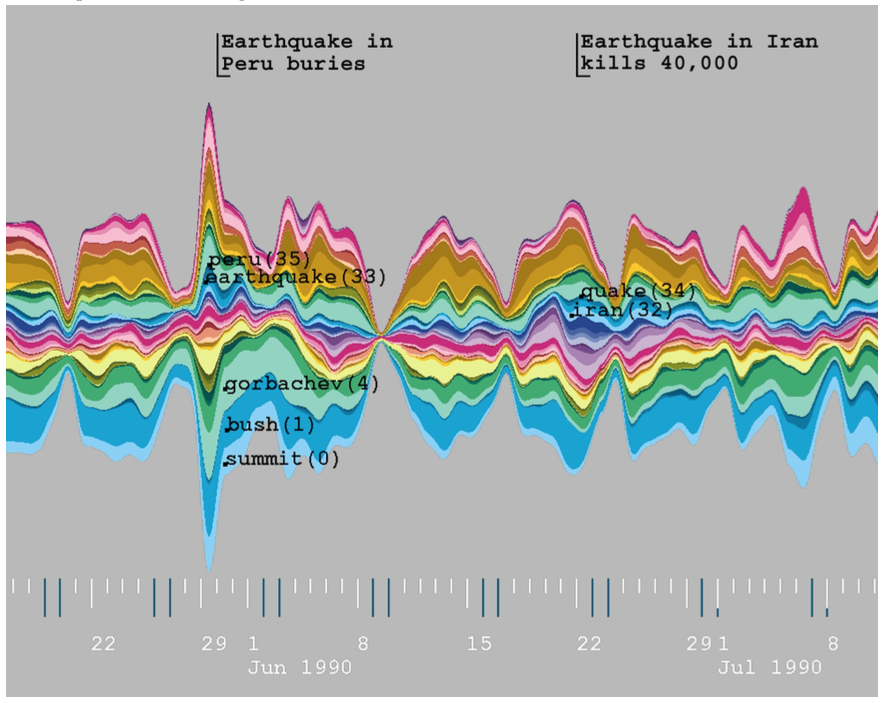
\includegraphics[width=.9\linewidth]{img/lit-survey/histogram1.png}
  \end{minipage}%
\begin{minipage}{.65\textwidth}
  \centering
  \hspace{-1.5cm}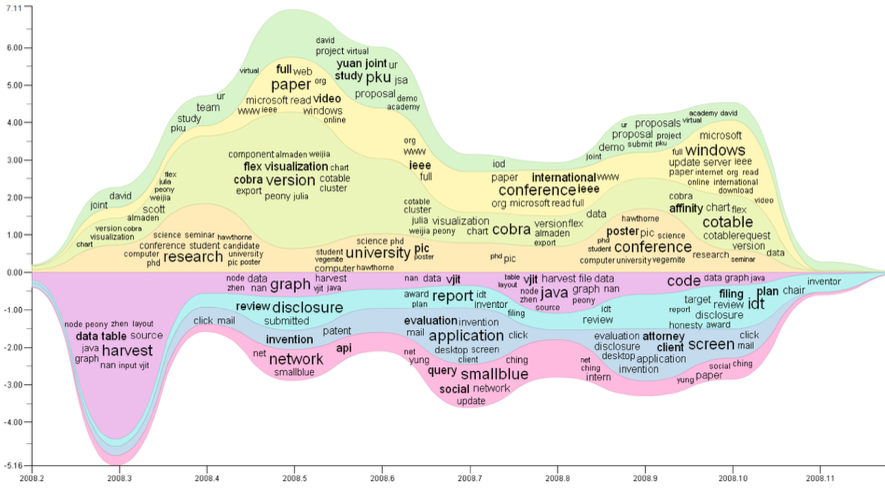
\includegraphics[width=.9\linewidth]{img/lit-survey/histogram2.png}
\end{minipage}
\caption{Similar visualisations from ThemeRiver \citep{ThemeRiver} (left) and TIARA \citep{InteractiveTopicBasedVisualTextSummarizationAndAnalysis} (right).}
  \label{fig:themeriver-tiara}
\end{figure}

Both ESTHETE \citep{ESTHETE} and nReader \citep{Nreader} present timeline-centric views for collections of news articles based on underlying graphs of relationships between the articles. However, in both cases, the graph structure was not part of the final visualisation, so connections between entities were displayed in purely textual forms. In contrast, ThemeRiver \citep{ThemeRiver} introduces a novel view on topic frequency along the time axis to show thematic change over time within a collection of documents, similar to a smoothed histogram. This view, while useful for large document collections which span weeks or months, would be less suited to displaying emerging news trends over shorter periods.

TIARA \citep{InteractiveTopicBasedVisualTextSummarizationAndAnalysis} whose authors cite ThemeRiver as an influencing design (see figure \ref{fig:themeriver-tiara}), displays a similar shaped graphical output but performs more detailed textual analysis, and displays related keywords in the output. Both visualisations support simple zooming and panning, but suffer from the same limitations on visualising topic connectivity as \citep{TimeSets}.

Taking into consideration both the critiques of  oversimplification identified in \citep{SchemaLine} and the physical limitations highlighted in \citep{TimeSets, ThemeRiver}, it is clear that timelines may not be the most appropriate visual metaphor for news visualisation, especially not for highly connected events and topics. However, for more linear storylines which span fewer categories or topics, a visualisation such as \citep{SchemaLine} could be used, for example as part of \citeauthor{TheEyesHaveIt}'s \textit{Zoom and Filter} task where the dataset is pruned.

\subsubsection{Topological and Schematic Map Visualisations}

The use of cartographic representations for abstract objects and the relationships between them is such a common and natural metaphor that it is often unnoticed in digital contexts. Maps take advantage of humans' natural ability to perceive and organise in a spatial context, and [the fact that we live in a spatial world] ``leads naturally to metaphors that provide cues for orientation and navigation'' \citep[p.2]{InformationCartographyUsingGIS}.

Topological maps\footnote{Not to be confused with \textit{topographic} maps, which represent relief and other geographic features of physical regions at a large scale and in fine detail.} are a specific class of map which abstract away detail so that only significant features within desired subsets of the mapped dataset remain; from a news overload perspective, this is a highly desirable property. These maps are often used to visualise networks and are represented as schematics, where elements on the map are transformed into abstract visual representations for ease of understanding. Today, the most recognisable examples of topological maps are transit maps. Divorced from the strictness of geographical accuracy and scale, emphasis is instead placed on the usability of the map for planning and the understanding of relative positioning which the maps enable \citep{TheInfluenceOfMapDesignOnRouteChoice}.

\begin{figure}[hp!]
	\centering
	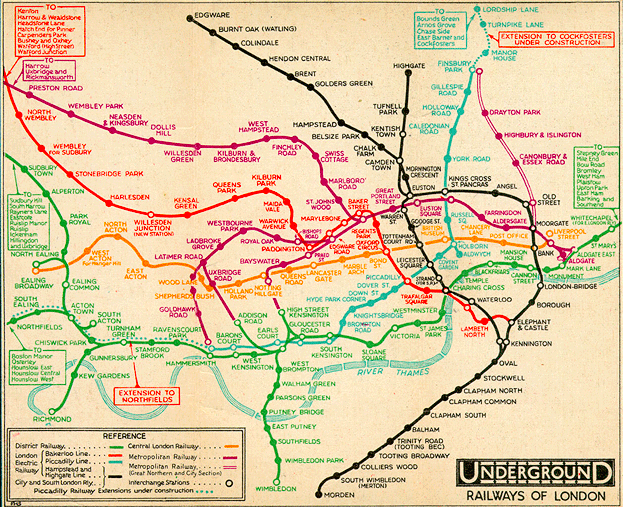
\includegraphics[width=.8\textwidth]{img/lit-survey/1930-pre-beck.png}
	\caption{1930 London Underground map, designed by F. Stingemore \citep{Tube150}.}
	\label{fig:pre-beck}
\end{figure}

\begin{figure}[hp!]
	\centering
	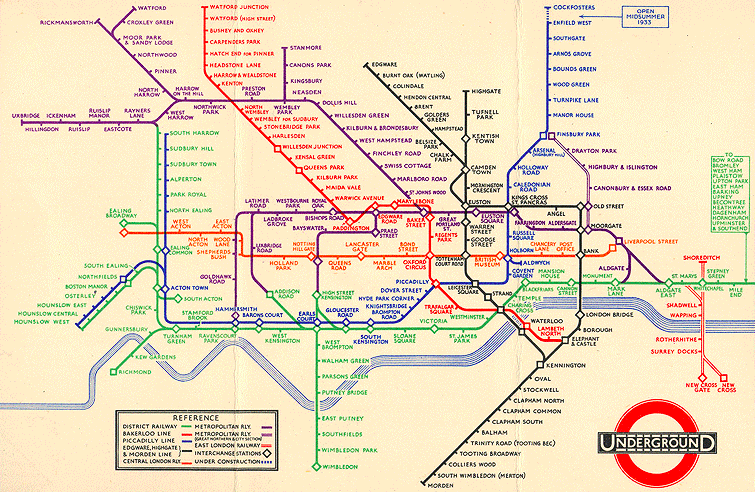
\includegraphics[width=.8\textwidth]{img/lit-survey/1933-beck.png}
	\caption{1933 London Underground Map, designed by H. Beck \citep{Tube150}.}
	\label{fig:beck}
\end{figure}

Figures \ref{fig:pre-beck} and \ref{fig:beck} show the geographically accurate 1930 London Underground map designed by Frederick Stingemore, and the iconic 1933 redesign by Henry Beck, which was based on the concept of an electrical circuit diagram \citep{HarryBeck}. While Beck's simplification of the structure of the map was seen as radical and even controversial at the time, the hallmarks of his design are now recognisable not just in other schematic maps, but in posters, infographics and diagrams across various domains.

In terms of usability, simple timeline visualisations can provide the chronological ordering which is intrinsic within collections of news articles. However, schematic maps may be able to represent complex relationships between topics in a structure which is linear but has an additional dimension, to prevent linearity becoming a design or usability constraint.

\section{Metro Maps for Information Cartography}
Significant work in the area of information cartography has been undertaken by Shahaf et al. \citep{ConnectingTheDots, GeneratingInformationMaps, MetroMapsOfScience, InformationCartographyPre}, in the domains of both news and science through the visualisation of article and journal data on metro maps.

\cite{GeneratingInformationMaps} chose the metaphor as a base for their visualisation to address the fact that previous timeline-based summarisation systems could only represent simple linear stories; ``In contrast, complex stories display a very non-linear structure: stories split into branches, side stories, dead ends, and intertwining narratives.'' \citep[p.1]{InformationCartographyPre}

\begin{figure}[htbp!]
	\centering
	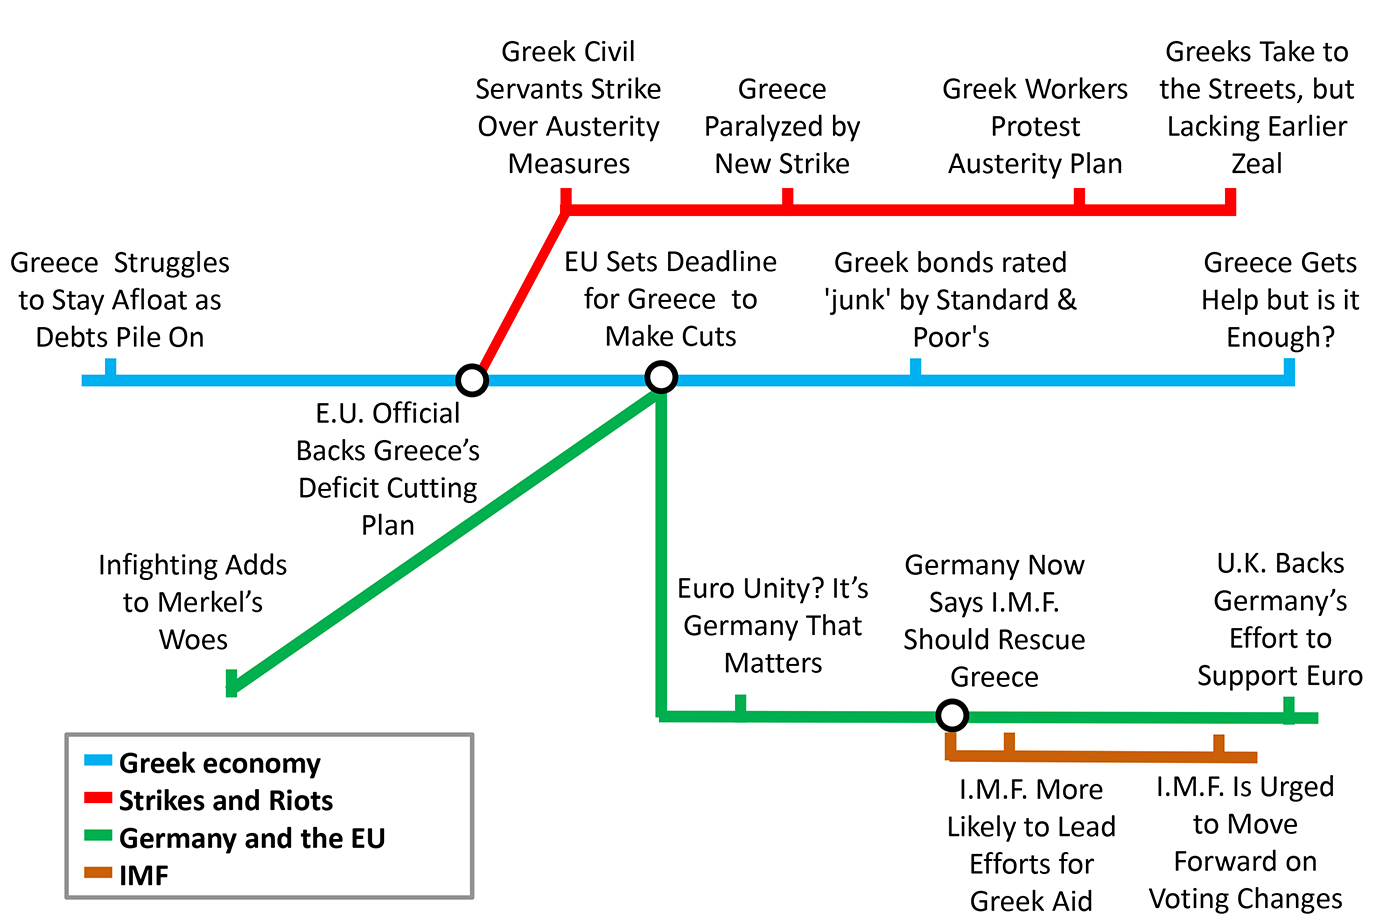
\includegraphics[width=.8\textwidth]{img/lit-survey/greece-metromap.jpg}
	\caption{A metro map \citep{GeneratingInformationMaps} covering the Greek Debt Crisis.}
	\label{fig:greecemetro}
\end{figure}

Even in a scientific context, this was not the first time the abstract visualisation potential of the metro map had been noted; ``The usefulness of the metro map as a metaphor is somewhat limited to simple examples by the time required to manually produce these maps. As such they are generally only useful for applications that do not change frequently. This limitation could be removed by quality methods for the automatic drawing of metro maps from abstract data.'' \citep[p.54]{AutomaticMetroMapLayoutThesis}

In this section, the formalisation of the metro map metaphor, its associated characteristics, and its limitations will be discussed.

\begin{definition}{Metro Map \citep{GeneratingInformationMaps}:}
A metro map $\mathcal{M}$ is a pair $(G, \Pi)$, where $G=(V, E)$ is a directed graph and $\Pi$ is a set of paths, or \textit{metro lines} in $G$. Each $e \in E$ must belong to at least one metro line.
\label{def:mm}
\end{definition}

A previously published method \citep{ConnectingTheDots} for linking together chains of articles  was discussed, and an objective function was created to formalise the characteristics of a `good' metro map. The function defined was a composite based on three important characteristics, all of which are broadly applicable to the visualisation of any similar corpora; coherence, coverage, and connectivity.

\subsection{Coherence}
Let $\mathcal{D}$ be a set of articles, and $\mathcal{W}$ be a set of words or phrases, such that each article is a subset of $\mathcal{W}$. A \textit{coherent} chain of articles through $\mathcal{D}$ is one where transitions between documents are smoothed by common overlapping keywords from $\mathcal{W}$, creating a better narrative flow \citep{ConnectingTheDots} as depicted in Figure \ref{fig:coverage}.

\begin{figure}[htbp!]
	\centering
	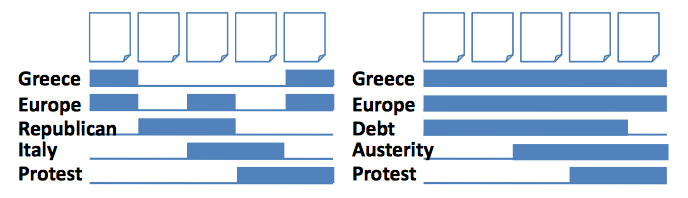
\includegraphics[width=.7\textwidth]{img/lit-survey/coverage.png} \par
	 A bar corresponds to the presence of a word in the article above it.\\The titles of the articles which made up the two chains were as follows:\\[0.2cm]\footnotesize{
	 \begin{tabular}{|l|l|}
	 	\hline 
	 	Chain A (left) & Chain B (right) \\
	 	\hline
	 	Europe weighs possibility of debt default in Greece & Europe weighs possibility of debt default in Greece \\
	 	Why Republicans don't fear a debt default & Europe commits to action on Greek debt \\
	 	Italy; The Pope's leaning toward Republican ideas & Europe union moves towards a bailout of Greece \\
	 	Italian-American groups protest `Sopranos' & Greece set to release austerity plan \\
	 	Greek workers protest austerity plan & Greek workers protest austerity plan \\
	 	\hline
	 \end{tabular}\vspace{0.2cm}}
	 \caption{An incoherent chain with jittery transitions between topics (Chain A, left) alongside a more coherent chain of articles (Chain B, right). \citep{GeneratingInformationMaps}}
	\label{fig:coverage}
\end{figure}

Coherence, intuitively, seems to be closely linked to idea of story resolution detailed in Section \ref{sec:information-overload}. This presents a question which could later be explored further; does forming coherent chains of articles provide the story resolution that participants in the Associated Press study were so desperately seeking from current events journalism?
	
\subsection{Coverage}
As in the previous section, let $\mathcal{D}$ be a set of articles, and $\mathcal{W}$ be a set of words or phrases of which the articles are composed. The coverage function for a word in a given document $d_i \in \mathcal{D}$ specified in Equation \ref{eqn:doc-coverage} can be quantified using any measure of how well $d_i$ covers $w$, for example tf-idf$(w, d_i, \mathcal{D})$ (See Equation \ref{eqn:tfidf}) \citep{GeneratingInformationMaps}.
\begin{equation}
	cover_{d_i}(w) : \mathcal{W} \rightarrow [0,1]
	\label{eqn:doc-coverage}
\end{equation}
Extending the notion of coverage to maps--which can be abstracted to sets of documents--introduces the idea of \textit{diversity}. If a map already contains documents which for a sufficient coverage for some word $w$, then there is nothing to be gained by adding another document to $\mathcal{D}$ which has high coverage of $w$ alone. This relates back to the principles of spatial and information quality discussed in Section \ref{sec:information-overload}, especially the importance of value-added by every individual document in a collection. In this case, maps which cover a maximal number of $w \in \mathcal{W}$ should be preferential. A simple additive definition for map coverage such as Equation \ref{eqn:additive-coverage} \citep{GeneratingInformationMaps} would not reward this kind of diversity;
\begin{equation}
	\label{eqn:additive-coverage}
	cover_\mathcal{M}(w) = \sum_{d_i\in docs(\mathcal{M})}cover_{d_i}(w)
\end{equation}
Therefore, an alternative definition for map coverage was chosen, which will not increase significantly if another document which covers an already covered feature is added to $\mathcal{D}$ (Equation \ref{eqn:multiplicative-coverage} \citep{GeneratingInformationMaps}).
\begin{equation}
	\label{eqn:multiplicative-coverage}
	cover_\mathcal{M}(w) = 1 - \prod_{d_i\in docs(\mathcal{M})}(1-cover_{d_i}(w))
\end{equation}
Finally, the definition of map coverage is extended to the coverage of the corpus $\mathcal{D}$, rather than just single features. If each feature is weighted according to frequency, then for each $w \in \mathcal{W}$ we have some $\lambda_w$. The coverage of a corpus $\mathcal{D}$ by a metro map $\mathcal{M}$ can then be defined as in Equation \ref{eqn:map-coverage} \citep{GeneratingInformationMaps}.
\begin{equation}
	\label{eqn:map-coverage}
	Cover(\mathcal{M}, \mathcal{D}) = \sum_{w \in \mathcal{W}}\lambda_w cover_\mathcal{M}(w)
\end{equation}

\subsection{Connectivity}
The final property is the most simply defined; the connectivity of a metro map is the number of paths in $\Pi$ which intersect \citep{GeneratingInformationMaps}.
\begin{equation}
	Connectivity(\mathcal{M}) = \sum_{i<j}\mathbbm{1}(p_i \cap p_j \neq\emptyset)
\end{equation}

\subsection{Limitations of \cite{GeneratingInformationMaps, InformationCartographyPre}}

\subsubsection{Corpus}
Perhaps the biggest limitation of the system developed in \citep{GeneratingInformationMaps, InformationCartographyPre} is the nature of the corpus $\mathcal{D}$; it is a fixed dataset, meaning users can only query it for certain past events with no way of specifying a different corpus themselves.

From a historical reference perspective the output generated based on certain queries is interesting when compared to the output an expert would select as important to the narrative, but it is not possible to use the system as a replacement to a newsfeed aggregator.

\subsubsection{Graph Layout Aesthetic Principles}

From a usability perspective, a second limitation of the work of \citeauthor{GeneratingInformationMaps} is the lack of focus given to the desirable aesthetic properties of transit maps.

A formative empirical study \citep{TheBasisForGraphDrawingAlgorithms} on how graph layout affects usability identified a collection of five measurable aesthetic principles from previous research, which aid human understanding when reading graphs:
\begin{itemize}[noitemsep]
	\item Minimise the number of line bends \citep{MinimiseBends};
	\item Minimise the number of edge crossings \citep{MinimiseEdgeCrossings};
	\item Preserve any underlying symmetry in the structure of the graph \citep{PreserveSymmetry};
	\item Draw orthogonally where possible \citep{MinimiseBends};
	\item Maximise the minimum angle between incident edges for each node \citep{IncidentEdges}.
\end{itemize}
These criteria, when numerically calculated and weighted relative to one another, allow the aesthetic quality of any graph to be evaluated. This is particularly useful for graphs generated by automatic layout algorithms, which aren't as much a product of human design intuition as their manually designed counterparts.

The origins of the principles above predate much of the early InfoVis research because several of them \citep{MinimiseBends, MinimiseEdgeCrossings} were formalised as guidelines for the design of electronic circuits.

In a later study, \citeauthor{WhichAesthetic} evaluated information-finding task performance with a set of graphs which varied the above principles, to establish which the most and least significant aesthetics were for graph usability. The results of the study were that maximising incident edge angles and orthogonality did not lead to better performance, preserving symmetry and minimising line bends were somewhat important, and minimising edge crossings was the most significant influencing factor for performance \citep{WhichAesthetic}. 
 
Metro maps, however--particularly those representing non-physical data such as in the previous section--do not share all the structural principles of the wider set of directed graphs. Consequentially, \citeauthor{AutomaticMetroMapLayout} developed a set of criteria for metro maps specifically, including criteria for the labelling of stations. The criteria are as follows \citep{AutomaticMetroMapLayout}:

\begin{itemize}
	\item \textbf{Angular Resolution Criterion:} Maximise the angle between incident edges at each node. This criterion is also the fifth principle in \citep{TheBasisForGraphDrawingAlgorithms}. 
	\item \textbf{Edge Length Criterion:} All edges on the map should be approximately equal.
	\item \textbf{Balanced Edge Length Criterion:} The length of edges incident to a given node should be approximately equal.
	\item \textbf{Edge Crossings Criterion:} Crossings should be minimised. This criterion is also the second principle in \citep{TheBasisForGraphDrawingAlgorithms}, also identified as the most important.
	\item \textbf{Line Straightness Criterion:} Edges on the same metro line should be collinear, i.e. they should form a 180$^{\circ}$ line through every station that the line passes through. This criterion relates closely to the first principle in \citep{TheBasisForGraphDrawingAlgorithms}.
	\item \textbf{Octilinearity Criterion:} Edges should be drawn at multiples of 45$^{\circ}$. This criterion is an extension to the fourth principle in \citep{TheBasisForGraphDrawingAlgorithms}, as orthogonality is here analogous to rectilinearity.
\end{itemize}

Evaluating Figure \ref{fig:greecemetro} according to the list above, we observe that despite only containing 16 stations, the map unnecessarily violates five  of \citeauthor{AutomaticMetroMapLayout}'s six criteria--all except edge crossings.

Therefore, to improve the usability of the metro maps drawn in \citep{ConnectingTheDots, GeneratingInformationMaps, MetroMapsOfScience, InformationCartographyPre}, it would be advisable to attempt to satisfy more of the aesthetic principles for graphs and metro maps described in \citep{TheBasisForGraphDrawingAlgorithms, AutomaticMetroMapLayout}.


\section{Towards Newsfeed Visualisation}

The fact that news articles form a fairly narrow class of document is an advantage from a visualisation design perspective, due to the common elements they share. Articles published by commercial news producers typically contain:
\begin{itemize}[noitemsep]
	\item A headline;
	\item A description, or \textit{subhead};
	\item A publish date;
	\item One or more categories to which the article belongs.
\end{itemize}
These attributes are useful for visualisation, since creating a spatial representation from text requires documents to be represented as vectors in high-dimensional feature space \citep{VisualizingTheNonVisual}, and the presence of existing attributes makes articles more inherently comparable than their unstructured contents would be.

There is also a well-known existing standard for publishing links to articles with their metadata for use by other applications; RSS.

\subsection{Content Retrieval}
The de-facto web format for feed publishing is RSS (Rich Site Summary, or Really Simple Syndication.) The rise of the internet as a news platform has lead to many readers finding the most efficient method of reading news articles is to subscribe to various topic-specific newsfeeds and read what is automatically collated by their computers \citep{Nreader}.

Although RSS--which is a subset of XML--is standardised\footnote{\url{http://cyber.harvard.edu/rss/rss.html}}, the practice of feed categorisation is not, meaning the granularity of topics which can be subscribed to is dependent on the publisher. This issue was addressed by \citet{PersonalNewsRss}, with the design of a system which could essentially split or join existing RSS feeds to synthesise new ones based on user-specified keywords and queries.

Despite its shortcomings, RSS remains the most universal option for accessing feed content from a wide variety of news producers 
\citep{MiningAndVisualisingInformationFromRSSFeeds}.

\subsection{Keyword Extraction}

Extracting relevant keywords from documents is not a new domain of research. Various methods have been presented, the most well-known being the intuitively logical tf-idf (term frequency, inverse document frequency) \citep{TermWeightingApproachesInAutomaticTextRetrieval} which ranks the significance of a term \textit{t} in a document \textit{d} which belongs to a corpus \textit{C} as follows:

\begin{equation}
	\text{tf-idf}(t) = \frac{Occurrences(t, d)}{WordCount(d)} \times log_e\bigg(\frac{|C|}{|\{c \in C \mid t \in c\}|}\bigg)
\label{eqn:tfidf}
\end{equation}

tf-idf will extract the most unique keywords from a document within a corpus, because it penalises words which are common to many documents. However, in the context of a corpus of news articles, this uniqueness can lead to significant topic keywords being ignored because they appear with such frequency. 

\citet{TopicExtractionfromnewsArchiveUsingTFPDFAlgorithm} found that for news archive keyword extraction, a better alternative to tf-idf is tf-pdf (term frequency, proportional document frequency) as it is not biased against frequently repeated keywords.

Using tf-pdf, articles are modelled as belonging to one of a finite number of sources or \textit{channels} within a corpus. The weighting of a term from an article within a channel is in this case linearly proportional to its frequency in the channel and exponentially proportional to the number documents in the channel where it occurs. A term's total weighting is the sum of its weightings across all channels, as can be seen in Equation \ref{eqn:tfpdf} \citep{TopicExtractionfromnewsArchiveUsingTFPDFAlgorithm}, where:
\begin{itemize}[noitemsep]
	\item $D$ = The number of channels in the corpus;
	\item $K_c$ = The total number of terms in channel $c$;
	\item $F_{tc}$ = Frequency of term $t$ in channel $c$;
	\item $n_{tc}$ = The number of articles in channel $c$ where term $t$ occurs;
	\item $N_c$ = The total number of articles in channel $c$.
\end{itemize}
\begin{equation}
	\label{eqn:tfpdf}
	\text{tf-pdf}(t, D, K) = \sum_{c=1}^{c=D}\frac{F_{tc}}{\sqrt{\;\sum\limits_{k=1}^{k={K_c}}{F_{kc}}^2}}\times\text{exp}{\bigg(\frac{n_{tc}}{Nc}\bigg)}
\end{equation}

The reliance of both tf-idf and tf-pdf on a fixed background corpus results in a need to recompute the function for every document if any are added to or removed from the collection. This is impractical for large collections, and even in the case of large fixed collections it does not scale well, which has resulted in the development of other methods.

An approach derived from energy levels in quantum systems was proposed in \cite{LevelStatisticsOfWords}, where keywords were extracted based on their spatial distributions within a single text. The theory behind the approach is that typically, keywords occurrences are distributed in significant frequency clusters throughout a document, whereas non-relevant words are distributed with uniform frequency (see Figure \ref{fig:ols-spectra}).

\begin{figure}[htbp!]
	\centering
	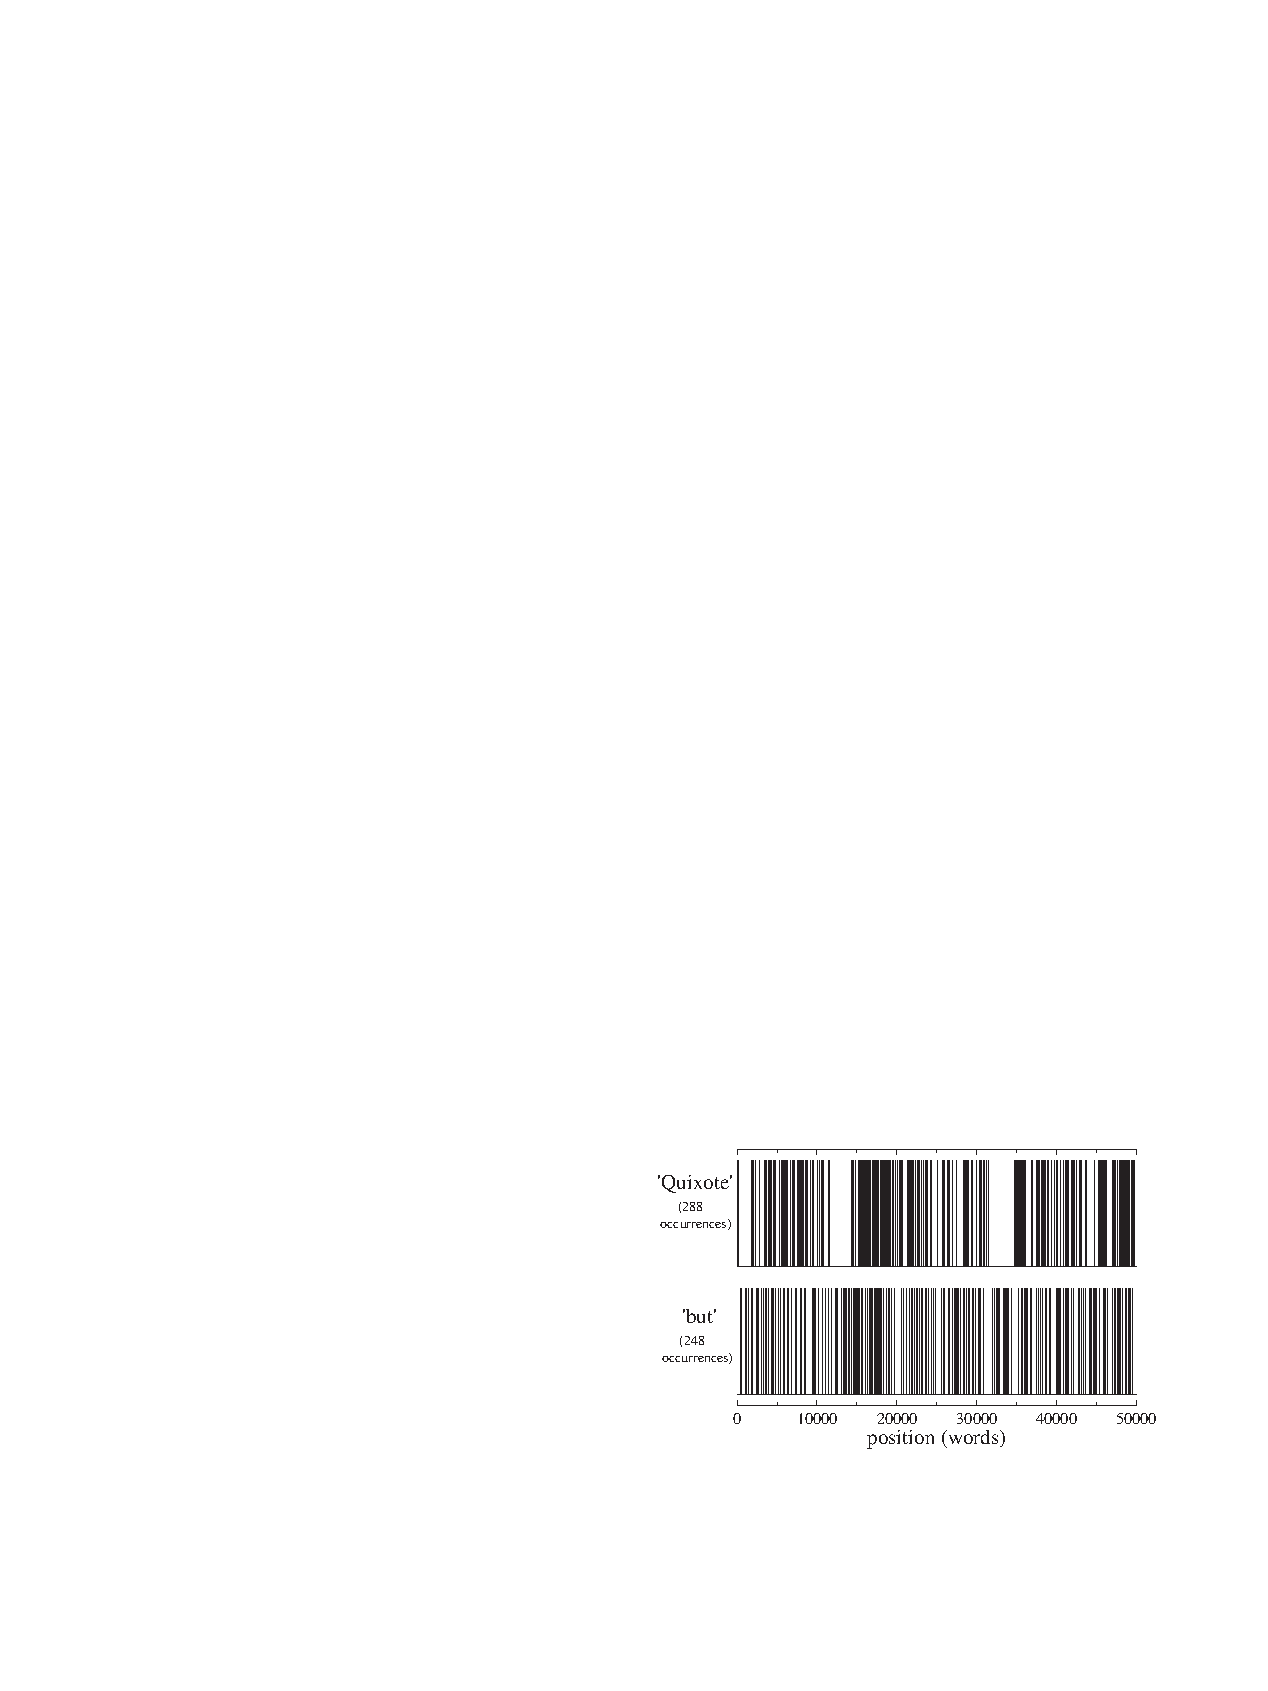
\includegraphics[width=.6\textwidth]{img/lit-survey/ols-keyword-spectra.pdf}
	\caption{Frequency spectra for `Quixote' and `but' in the first 50,000 words of \textit{Don Quixote}. \citep{LevelStatisticsOfWords}}
	\label{fig:ols-spectra}
\end{figure}

This technique allows relevant keywords to be distinguished from non-relevant common words with similar total frequencies without the use of a background corpus for comparison.

Several important observations have been made regarding keyword extraction for news articles specifically. Firstly, that important phrases in text are likely to be references to people, places and other named entities \citep{NewsStand}. Libraries such as the Stanford Named Entity Recognizer (NER) \citep{NestedNamedEntityRecognition} exist to extract these from text. 

Secondly, that while 30\% of an article's keywords are inferred and cannot be found within the text without intelligent input, 60\% are present in the article's title and first few sentences \citep{IdentifyingTopicsByPosition}, since important facts are generally stated as part of an article's \textit{above the fold} content.

\section{Evaluation Methods}
\citet{GeneratingInformationMaps} evaluated their system both for accuracy and with a user study, though as previously discussed they did not evaluate the aesthetic properties of the generated maps. The accuracy evaluation tested whether the system included the most `important' (as decided by experts) documents in the map. 

The user study focused on the strength of the results returned by specific queries, where output was transformed into a structureless list in order for the study to be double-blind against the other methods. The evaluation was performed between-subjects, so background knowledge had to be controlled for. Output was compared with that from Google News and a TDT (Topic Detection and Tracking) method presented in \citep{SemanticLanguageModelsForTDT}. 

This approach to evaluation is less relevant to my proposed system, since it was actually evaluating the performance of the system in selecting documents based on a query, rather than visualising the documents on a map. In contrast, a visualisation and its usability is precisely the aspect of my process which I would need to evaluate.

%\citet{EvaluatingInformationVisualisations} found that the evaluation of measures of usability such as task completion time and effectiveness can only be accurately conducted as part of a summative formal experiment. This is because formative tests such as think-aloud experiments require users to alter their behaviour and leads to slower actions \citep{VerbalReportsAsData}.

The evaluation of TIARA \citep{InteractiveTopicBasedVisualTextSummarizationAndAnalysis} was a more relevant method than the Metro Map evaluation as it was conducted against a baseline system which did not share any of its advanced features, although it was tailored for the same task; email analysis. A series of questions were asked of participants, who used either TIARA or the baseline system to answer. The response time and accuracy of the participants was recorded, as well as their levels of satisfaction after completing the task. This evaluation used between-subjects designs and therefore required the use of a different dataset for each task, as the nature of the sensemaking means any repetition of the evaluation task on the same data would see participants' performance improve significantly due to recall alone.

\section{Summary}

To recap, this review began with an exploration of the problem of news overload using the findings of The \cite{anewmodelfornews}, a field study conducted into the news consumption habits of young people. The findings of the study were then discussed, firstly in the context of four dimensions of information overload \citep{TowardsAnOptimalResolutionToInformationOverload, GuestEditorsIntroductionInformationOverload} and secondly in terms of how they relate to sensemaking; the cognitive process this project aims to support.

Information visualisation was identified as one common approach to both support sensemaking and reduce information overload, so various methods for visualising text-based documents and news articles specifically were presented and compared \citep{ESTHETE, ThemeRiver, InteractiveTopicBasedVisualTextSummarizationAndAnalysis, ExploringLongRunningNewsStoriesUsingWikipedia, Nreader} as well as a more in-depth exploration of visual metaphors, in particular timeline, and schematic map visualisations. This section also featured the introduction of the metro map in its original context, before moving on to its use as a metaphor for visualisation in various domains.

Centrally, the work of Shahaf et al. \citep{ConnectingTheDots, GeneratingInformationMaps, MetroMapsOfScience, InformationCartographyPre} which is particularly relevant to the aims and objectives of this project was discussed in detail, with an explanation of key metrics (\textit{coherence}, \textit{coverage} and \textit{complexity}) defined in \citep{GeneratingInformationMaps} which are applicable to all graph-based representations of document collections. My main critiques of this body of work were the fixed background corpus and the physical layouts of the drawn maps when evaluated against the criteria defined in \citep{TheBasisForGraphDrawingAlgorithms, AutomaticMetroMapLayout}.

Next followed a practical overview of methods for transforming news articles into entities with visual or comparative properties, including RSS feed mining, entity recognition, and keyword extraction. Lastly, approaches to experimental design and evaluation by several of the aforementioned studies were discussed in the context of their relevance to the proposed system. 

The background, techniques and terminology discussed in this review will be taken forward into the next chapters, as they were all at least partially influential in the design and implementation of the system.
This is the chapter for your Literature Survey.

You will wish to cite authors like \cite{latex} or \cite{btxdoc}.  Alternate
commands are used to cite \citeasnoun{latex} as a noun, or cite
\possessivecite{latex} work possessively, or add text to the citation, 
\citeaffixed{latex}{e.g.}.

If these citations do not compile correctly, ensure you have the Harvard
package installed.  You can pick up the Harvard package in the zip file
of the dissertation template files you downloaded.


%%
%% NOTE: Replace the following with chapters that are appropriate for your
%%       style of project.  It is unlikely these will fit your project perfectly.
%%

\chapter{Requirements}
If you are doing a primarily software development project, this is the
chapter in which you review the requirements decisions and
critique the requirements process.


\chapter{Design}
This is the chapter in which you review your design decisions at various
levels and critique the design process.


\chapter{Implementation and Testing}
This is the chapter in which you review the implementation and testing
decisions and issues, and critique these processes.

Code can be output inline using \verb@\lstinline|some code|@.  For example,
this code is inline: \lstinline|public static int example = 0;|  (I have
used the character \verb@|@ as a delimiter, but any non-reserved character
not in the code text can be used.)

Code snippets can be output using the \verb|\begin{lstlisting} ... \end{lstlisting}|
environment with the code given in the environment.  For
example, consider listing \ref{Example-Code}, below.

\begin{lstlisting}[breaklines,breakatwhitespace,caption={Example code},label=Example-Code]
public static void main() {

  System.out.println("Hello World");

}
\end{lstlisting}

Code listings are produced using the package ``Listings''.  This has many
useful options, so have a look at the package documentation for further
ideas.


\chapter{Results}
This is the chapter in which you review the outcomes, and
critique the outcomes process.  You may include user evaluation here
too.


%%
%% Now we are back to the standard project contents that you should include
%%

\chapter*{Conclusions}
%The following chapter outlines the contributions of this work and the limitations of both our system and evaluation. It also describes extensions which could be developed given additional time, and areas which would benefit from further research.

\section{Summary of Contributions}

This dissertation introduced the first application of the metro map metaphor \citep{GeneratingInformationMaps} to news corpora extracted from user-specified RSS feeds, in order to automatically generate structured topic maps based on current events news. These metro maps serve as an effective comprehension aid to young people in our current digital landscape of news overload; a claim which we are the first to evaluate via direct comparison or our system with a typical RSS feed reader.

Our implementation includes a novel keyword extraction algorithm which performs keyword boosting using a knowledge base for entity disambiguation, and is tuned specifically for extracting entities from current events news. In the subdomain of metro map topology, our method also formalises \textit{Line Coverage} and \textit{Affinity} as an extension to the characteristics defined by \cite{GeneratingInformationMaps}, which can be used to compare the quality of candidate lines during the selection and pruning processes.

Due to the lack of any existing library for positioning or drawing metro maps, further contributions made include recommendations on tuning specific D3.js parameters within a force-directed layout to generate viable starting positions for stations on a metro map, and notes on the implementation of functions to calculate \possessivecite{AutomaticMetroMapLayoutThesis} line straightness and octilinearity criteria in JavaScript. To the best of our knowledge, this is the first application of \citeauthor{AutomaticMetroMapLayoutThesis}'s aesthetic criteria for metro map layout optimisation to non-geospatial maps.

The final contribution of this work is an empirical evaluation of the task performance of young adults using the system. The results of our experiments support our hypothesis that users recall more news topics from a news corpus using our metro maps than after using an unstructured RSS feed reader, and therefore substantiate our recommendations that future efforts to support the contextual linking of news articles should look to visualisation and cartography for direction.

\section{Limitations}

The main limitation of this work is the lack of a formal deterministic algorithm for drawing metro maps, using D3 or otherwise. The approach presented in Section \ref{sec:drawing} is nondeterministic by necessity in order to generate initial starting positions which result in few or no edge crossings, but this process is non-convergent and often results in suboptimal embeddings, the worst cases of which are unusable. 

As a result of this limitation, a significant effort was made to decouple the map drawing process from the other components of the system, such that it could be improved or replaced in future with the only changes required being to the interface at the serialisation stage. While the problem of generating planar embeddings for metro maps is known to be NP-hard, the maps drawn by our system are typically significantly smaller than metro maps which represent real existing transit networks, meaning it would not be unrealistic to use a non-polynomial time algorithm.

A second important limitation of the system is the inability of the graph formation logic to recognised an overly sparse, overly connected, or overly populated map. All three of these properties are easily addressed in theory; an overly sparse graph should trigger a repeat of the keyword extraction process with a larger keyword vector per article, an overly connected graph should trigger a repeat of the same process with a smaller keyword vector per article, and an overly populated map should use both a smaller keyword vector and have its lowest ranking metro lines removed. However, in the given time, it was not possible to implement this logic in the system, resulting in a need to manually tune parameters such as the above during its operation.

In terms of experimental design, the the weaknesses of this work lie in its limited scope. While our user study managed to capture a wide range of news consumption behaviours and attitudes among participants, all participants were students aged 20-23 who were technically proficient. 15 out of the 16 were Computer Science undergraduates, who are typically more familiar with graph theory and therefore more confident interpreting representations of abstract graphs than the general young adult population. This is a limitation which could be addressed by further experiments, as although the system was conceptualised for use by young adults as a result of The \possessivecite{anewmodelfornews} findings, it would have strengthened our conclusions to have evaluated the system in a larger study of both adults adults over the age of 25, and teenagers, especially those from a non-scientific background.

In addition to the lack of participant academic diversity, the scope of our measurement of task performance could also have been extended. The study we conducted was focussed exclusively on recall, but this recall is only one of the six factors identified by \cite{VisuelleKommunikation} as being strengthened by the use of visual metaphors, the others being motivation, the formation of new perspectives, support for learning, focusing of attention, and structuring of communication. It could be argued that the act of creating a topic index also evaluated the structure of participants' communication, but this still leaves four factors remaining.  

A more long-term study could have evaluated whether the daily use of metro maps supported participants' learning and/or increased their motivation to read the news, as these were the two factors identified in Chapter \ref{c:litreview} as the most critical influencers of news fatigue.


\section{Directions for Future Research}

This section outlines areas we consider to be of interest for future work on the basis of this dissertation.

\subsection{Real-Time News Tracking for Automated Collation}

If the system were developed to a stage where no manual tuning was required to prune the candidate metro lines to a level which struck a balance between useful and usable, article collation would a simple process to automate, meaning maps could be automatically generated on a periodic basis with no need for user input.

Web services such as News API \footnote{\url{https://newsapi.org}}, which publish a continual stream of JSON metadata containing live headlines from 72 major worldwide news publishers, are gaining traction as the demand for immediate information increases. Although metro maps have not been designed with live updating in mind, the use of services such as News API could serve as a replacement for specific RSS feeds, removing the major initial parameter of the system.

The key questions posed by the concept of real-time metro maps of news are related to the mechanics of updating, and how stateful the updates should be. Should the publishing of ten new headlines trigger a complete regeneration of the map (which would potentially result in a new set of metro lines) or should metro lines be fixed over a specific period of time? Would users want to be able to `pin' metro lines to indicate that the system should consider this an ongoing topic of interest and always choose it as a candidate?

We suspect that there is a limitation on the usefulness of metro maps when their data is continually updating in real-time due to the structural changes which could occur within the maps, but the core idea of dispensing with specific RSS feeds and simply watching major news outlets for trends is an interesting one. While users may find it beneficial to combatting news fatigue to specify exactly where they want their news to originate from or which topics they want to read about, real-time headlines also take the effort out of specifying feeds for users who are indifferent about the sources of the news they consume.


\subsubsection{Social Media Trending Topics}

In the current information landscape, it is impossible to discuss real-time news publishing without touching on social networks. The evolution of social media websites -- in particular, Twitter -- has been instrumental in the erosion of the dichotomy between news media and social networking websites. The majority of people receive personalised news recommendations every time we open Facebook or Twitter, sometimes without realising that their personal data and browsing histories are being used to construct these recommendations.




\subsection{Verification of News}





This is the chapter in which you review the major achievements in the
light of your original objectives, critique the process, critique your
own learning and identify possible future work.


\bibliography{Bibliography.bib}

\appendix

\chapter*{Design Diagrams}

\chapter*{User Documentation}

\chapter*{Raw results output}

\chapter*{Code}


\begin{landscape}
\begin{multicols}{2}
\section{File: yourCodeFile.java}
\lstinputlisting[basicstyle=\scriptsize]{yourCodeFile.java}
\end{multicols}
\end{landscape}

\end{document}
